 
To solve the problem of non-invertibility we couple the network weakly to the global reference pitch, as indicated at the bottom of Fig.~\ref{circuit}. This amounts to adding the term to the potential~(\ref{GeneralV})
%
\begin{equation}
V[\vec\lambda] \;=\; \frac14 \sum_{i,j=1}^N w_{ij} \Bigl( \lambda_j(t)-\lambda_i(t)-\phi^\JI_{ij}\Bigr)^2 \,+\,
\frac \epsilon 2 \sum_{i=1}^N ( \lambda_i - \lambda_\REF)^2\,,
\end{equation}
%
where $\lambda_\REF = 1200 \log_2 (f_{k_0}/440$ Hz) is the deviation from the reference pitch and
$\epsilon \ll w_{ij}$ is a small coupling parameter, replacing Eqs. (\ref{AB}) and (\ref{C}) by the modified expressions
%
\begin{eqnarray}
\mathbf{A}_{ij} &=& \left\{
\begin{array}{cc}
-w_{ij} & \mbox{ if } i\neq j  \\
\epsilon + \sum_{\ell} w_{i\ell} & \mbox{ if } i=j 
\end{array} \right.
\\
b_i &=& - \epsilon \lambda_\REF + \sum_j w_{ij} \,\phi_{ij}
\\
c&=&\frac14 \Bigl( 2N \epsilon \lambda_\REF^2 + \sum_{i,j} w_{ij} \phi_{ij}^2\Bigr) \,.
\end{eqnarray}
%
Now the matrix $\mathbf A$ is invertible and the optimal pitch differences can be computed by $\vec\lambda^\OPT=-\mathbf{A}^{-1}\vec b$. A similar modification can be made if horizontal tuning is taken into account.



%==========================================================================
\section{Appendix: Tuning Module -- Technical Details}
%==========================================================================

In the source code, which can be downloaded from \href{https://gitlab.com/tp3/JustIntonation}{\tt https://gitlab.com/tp3/JustIntonation}, the core of the tuning module can be found in the directory {\tt ./application/modules/tuner}. The tuner interface is realized as an instance of the class {\tt Tuner} which is in turn running an instance of the {\tt TunerAlgorithm} in an independent thread. 

%------------------------------------------------------------------------
\begin{figure}[t]
\centering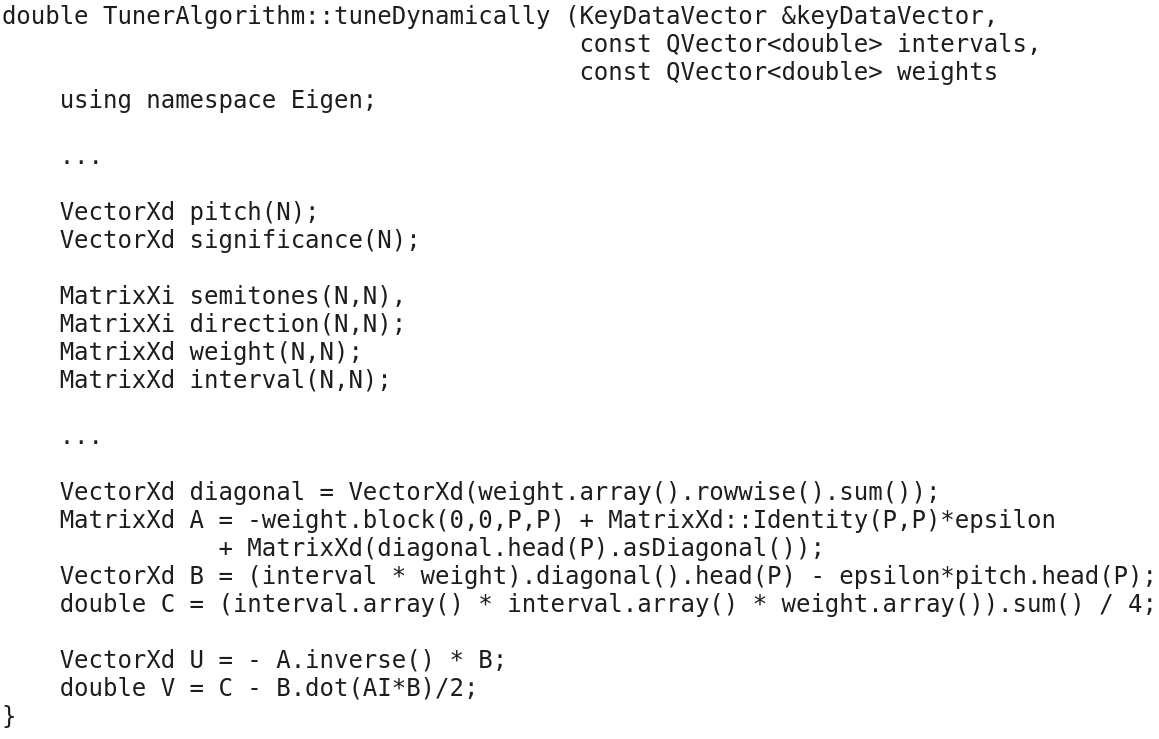
\includegraphics[width=150mm]{code}
\caption{Code excerpt from the tuning module (see text).\label{code}}
\end{figure}
%------------------------------------------------------------------------

A greatly shortened excerpt of the main algorithm without optimization is shown in Fig.~\ref{code}. As can be seen, the function {\tt tuneDynamically} is called with three arguments, passing a structure containing the status of all keys, a vector of the desired interval sizes in cents, and a vector of the corresponding weights which can be adjusted individually in the expert mode of the application.

The implementation of the tuner algorithm is based on the open-source library,\footnote{Open-source software library for linear algebra, see \href{http://eigen.tuxfamily.org}{\tt eigen.tuxfamily.org}} a C++ library for linear algebra, which is used here to solve the system of linear equations described above. First two vectors and four matrices are declared and initialized as follows (the initialization is not shown in Fig.~\ref{code}):
%
\begin{itemize}
 \item {\tt pitch} is a vector containing the actual pitches of the pressed keys in cents.
 \item {\tt significance} is a vector holding the weight of each pressed key depending on its volume.
 \item {\tt semitones} is a matrix counting the number of semitones between each pair of the pressed keys.
 \item {\tt direction} indicates whether the corresponding interval goes up or down.
 \item {\tt weight} is an array containing the tuning weights according to the slider setting in the expert mode.
 \item {\tt interval} contains the desired JI interval sizes in cents.
\end{itemize}
After initializing these objects, we use the \textit{Eigen} library to set up $A,B$, and $C$ (see Fig.~\ref{code}) and finally we solve Eqs. (\ref{eqa})-(\ref{eqc}). The actual solution of the problem is carried out in a single line, namely

\begin{center}
{ \tt VectorXd U = - A.inverse() * B; }
\end{center}

For further details we refer the interested reader to the documentation of the source code on \href{http://doxygen.just-intonation.org}{\tt doxygen.just-intonation.org}.

